We will start this chapter with general considerations about systems of partial differential equations (basic definitions, existence theorem and the notion of characteristics). More specifically, it will be seen that partial differential equations of high order can be reduced to first order systems of partial differential equations, in which fall equations of dynamics in solid mechanics (see section \ref{sec:solidMech_equations}). Then, the general concepts introduced in section \ref{sec:PDEs} will be applied in the context of solid mechanics conservation laws (section \ref{sec:characteristic_analysis}) in order to derive analytical solutions of one-dimensional problems in section \ref{sec:analytical_results}.
\subsection{General concepts}
A \textit{system of partial differential equations} can be written by means of a vector operator $\vect{\Fc}$ of independent and dependent variables $(x_1,...,x_N)$ and $(u_1,...,u_I)$:
\begin{equation}
  \label{eq:diff_operator}
  \vect{\Fc}\(x_1,...,x_N,u_1,...,u_I,\drond{u_1}{x_1},..., \drond{^Mu_I}{x_N^M}\) = \vect{0}
\end{equation}
The dimension of the system is given by the size of the array $\vect{\Uc}^T=[u_1,...,u_I] \in \Rbb^I$, also referred to as the \textit{unknown vector}. The highest derivative of the unknown vector in the system defines the \textit{order of the system}. In equation \eqref{eq:diff_operator} and in what follows, sans-serif symbols refer to matrices while calligraphic symbols stand for column array. Furthermore, the partial derivatives of a quantity $u$ with respect to a variable $x$ may be replaced by $u_x$ when there will be no ambiguity. Making use of index notation and convention of implicit summation over repeated indices, a system of partial differential equations can be written:
\begin{equation*}
  \sum_{k=1}^{N}\Asf_{ij}^p \drond{^p\Uc_j}{x_k^p} + \Bc_i = 0
\end{equation*}
or equivalently, in matrix form:
\begin{equation}
  \label{eq:diff_system_matrix}
  \sum_{k=1}^{N}\tens{\Asf}^p \drond{^p\vect{\Uc}}{x_k^p} + \vect{\Bc} =  \vect{0}
\end{equation}
Coefficients matrices $\tens{\Asf}^p$ and the vector $\vect{\Bc}$ may be functions of independent variables and the unknowns vector ($x_1,...,x_N,\vect{\Uc}$) leading to different types of partial differential systems. Namely, whether those terms are functions of the $x_k$ are not leads respectively to a \textit{linear system with variable coefficients} or to a \textit{linear system with constant coefficients}. The system remains \textit{linear} if $\vect{\Bc}$ depends linearly on $\vect{\Uc}$, and is \textit{semi-linear} if the relation is non-linear. Finally, if $\tens{\Asf}^p$ depends on independent variables, $\vect{\Uc}$ and its derivatives up to order $M-1$, the system is called \textit{quasi-linear}.


The \textit{Initial Value Problem (IVP)} or \textit{Cauchy problem} consists in finding a solution $\vect{\Uc}$ of system \eqref{eq:diff_system_matrix} that satisfies a set of given initial conditions. Geometrically speaking, the solution of such a problem can be seen as the building of an hyper-surface surface of $\Rbb^{I+N}$, hence the term of \textit{integral surface} for $\vect{\Uc}$. Such a problem can be reduced to that of solving a first order IVP by using suitable change of variable. To illustrate this property of PDEs, we consider a second order partial differential equation of two independent variables $(x,y)$ for the unknown $u$:
\begin{equation}
  \label{eq:2nd_order_pde}
  F(x,y,u,u_x,u_y,u_{xx},u_{yy},u_{xy})=0
\end{equation}
It is assumed that is equation can be rewritten as:
\begin{equation}
  \label{eq:2nd_order_pde_normal}
  u_{xx}= f(x,y,u,u_x,u_y,u_{yy},u_{xy})
\end{equation}
with associated initial conditions:
\begin{equation}
  \label{eq:2nd_order_pde_ICs}
  u(0,y)= g(y) \quad ; \quad u_x(0,y)= g_1(y)
\end{equation}
Then, applying the following change of variables:
\begin{equation*}
  \label{eq:change_of_variables}
  p = u_x \quad  ; \quad   q = u_{y}  \quad   ; \quad    r = u_{xx} \quad   ; \quad  s = u_{yy} \quad;\quad   t = u_{xy} 
\end{equation*}
and differentiating equation \eqref{eq:2nd_order_pde_normal} with respect to $x$:
\begin{equation*}
  \label{eq:r_x}
  u_{xxx}= f_x + f_u u_x + f_{u_x}u_{xx} + f_{u_y}u_{yx} + f_{u_{yy}}u_{yyx}+f_{u_{yx}}u_{yxx}
\end{equation*}
yields the following first order partial differential system:
\begin{equation}
  \label{eq:1st_order_quasi-linear_system}
  \begin{aligned}
    u_x  = p \quad & ; \quad    q_x  = p_y \\
    p_x  = r \quad &;\quad     t_x  = r_y \\
    s_x  = t_y \quad &;\quad   r_x  = f_x + f_up + f_p r + f_q p_y + f_s t_y + f_t r_y
  \end{aligned}
\end{equation}
Furthermore, from \eqref{eq:2nd_order_pde_ICs} and equation \eqref{eq:2nd_order_pde_normal}, initial conditions associated to system \eqref{eq:1st_order_quasi-linear_system} can be determined:
\begin{equation}
  \label{eq:1st_order_quasi-linear_system_ICs}
  \begin{aligned}
    u(0,y) = g(y) \quad & ; \quad     p(0,y) = g_1(y) \\
    q(0,y) = g'(y) \quad & ; \quad    s(0,y) = g''(y) \\
    t(0,y) = g_1'(y) \quad & ; \quad    r(0,y) = f(0,y,g(y),g_1(y),g'(y),g''(y),g_1'(y))
  \end{aligned}
\end{equation}
The solution of problem \eqref{eq:1st_order_quasi-linear_system}--\eqref{eq:1st_order_quasi-linear_system_ICs}  is equivalent to that of equation \eqref{eq:2nd_order_pde} and the procedure can be extended to more than two variables and higher orders \cite[p.54]{PDEs}. Note that the differentiation of the original PDE leads to a quasi-linear equation. Hence, such a reduction will yield a quasi-linear first order system regardless of the nature of initial equations.

\subsection{Notion of characteristics -- Hyperbolic problems}
The theorem of \textit{Cauchy--Kowalevsky} locally ensures the existence of solutions to a Cauchy problem for partial differential systems and is based on the restrictive requirement of analytic coefficients and initial data (see \cite[p.46]{PDEs}). The case of first order systems, however, only requires continuity and differentiability conditions and lies on the concept of \textit{characteristics}, which makes the development of a solution procedure more flexible.

\subsubsection*{First order quasi-linear equations}
We consider the first order quasi-linear PDE with independent variables $x$ and $t$:
\begin{equation}
  \label{eq:1st_order_pde}
   a u_x + b u_t  = c
\end{equation}
where coefficients $a$ and $b$ are such that $a^2 + b^2 \neq 0$. We prescribe initial values of $u$ along a curve $\Cscr_0$ in the $(x,t)$ plane defined as $\phi(x,t)=const$. The set $\phi(x,t),u\(\phi(x,t)\)$ thus defines a curve $\Cscr$ of the space $(x,t,u)$ which unique projection in the plane $u=0$ is $\Cscr_0$ (see figure \ref{fig:initial_curve}). Moreover, we assume that $\Cscr_0$ is regular, namely $\phi_x^2 + \phi_t^2 \neq 0$ and that, without loss of generality, one of the partial derivative does not vanish, say $\phi_\x \neq 0$.

\begin{figure}[h]
  \centering
  \begin{tikzpicture}
  \begin{axis}[view={30}{30},ticks=none,xlabel=$x$,ylabel=$t$,zlabel=$u$,zmin=0,ymax=5.2]
    \addplot3[Orange,very thick,domain=0:10,samples=60,samples y=0]
    ({x},
    {4+sin(1.5*x*x)},
    {4+3.*cos(deg(x))});
    \addplot3[Duck,dashed,very thick,domain=0:10,samples=60,samples y=0]
    ({x},{4+sin(1.5*x^2)},{0*x});
    \legend{$\Cscr$,$\Cscr_0$};
    % dt/dx = -phi_x/phi_t 
    \addplot3[thick]  coordinates {(5,4+sin(1.5*25),0) (6.5,4+sin(1.5*25),0)}  node[above] at (axis cs:6.9,4.05+0.6087-0.4,0.) {\large$\varphi_t$};
    \addplot3[thick]  coordinates {(5,4+sin(1.5*25),0) (6.5,4+sin(1.5*25)+0.3,0)};
    \addplot3[thick]  coordinates {(6.5,4+sin(1.5*25),0) (6.5,4+sin(1.5*25)+0.3,0)} node[right] at (axis cs:6.7,4.05+0.6087+0.,0.) {\large$-\varphi_x$};
  \end{axis}
\end{tikzpicture}
%%% Local Variables:
%%% mode: latex
%%% TeX-master: "../../mainManuscript"
%%% End:

  % \caption{Example of initial curve $\Cscr$ of the $(x,t,u)$ space and its projection $\Cscr_0$ in the $(x,t)$ plane with $\phi(x,t)=t-\sin(\frac{3x^2}{2})=0$.}
  \caption{Example of initial curve $\Cscr$ of the $(x,t,u)$ space and its projection $\Cscr_0$ in the $(x,t)$ plane.}
  \label{fig:initial_curve}
\end{figure}
With initial conditions given along $\Cscr$, the Cauchy problem is equivalent to that of finding a surface $u(x,t)$ that contains the initial curve and satisfies \eqref{eq:1st_order_pde}. Thus, one seeks the derivatives of $u$ along the initial curve. Since $u=u(\phi(x,t))$ along $\Cscr$, one can write:
\begin{equation*}
  u_x = u' \phi_x \quad ; \quad u_t = u' \phi_t
\end{equation*}
Substitution of $u'$ then leads to:
\begin{equation*}
  u_t = \frac{\phi_t}{\phi_x}u_x 
\end{equation*}
By using this relation between the derivatives of $u$ along $\Cscr$ in the PDE \eqref{eq:1st_order_pde}, one gets:
\begin{equation}
  \label{eq:normal_form_pde}
  (a + b\frac{\phi_t}{\phi_x})u_x = c
\end{equation}
Using the definition of the function $\phi(x,t)=const$ it comes:
\begin{equation*}
  d\phi = \phi_x dx + \phi_t dt =0
\end{equation*}
Finally with this consideration, equation \eqref{eq:normal_form_pde} can be rewritten as:
\begin{equation}
  \label{eq:normal_form_pde_2}
  (a - \ddroit{x}{t}b)u_x = c
\end{equation}
Thus, it is obvious that the Cauchy problem admits an unique solution if and only if
\begin{equation}
  \label{eq:non-characteristics}
  \ddroit{x}{t}\neq \frac{a}{b}
\end{equation}
If an initial curve satisfies the condition \eqref{eq:non-characteristics}, it is called a \textit{non-characteristic curves} or \textit{free curve}, otherwise it is a \textit{characteristic curve}. 

The concept of characteristics can be illustrated by looking at the set of solutions of equation \eqref{eq:1st_order_pde}. Indeed, those solutions $u^{(i)}(x,t)$ form a set of surfaces in the space $(x,t,u)$ which tangent planes have normal vectors $\vect{n}^{(i)}=[u^{(i)}_x,u^{(i)}_t,-1]$. According to equation \eqref{eq:1st_order_pde}, we see that these normal vectors are perpendicular to the vector $\vect{v}=[a,b,c]$. Therefore, the intersection of all those planes is a straight line which direction is given by $\vect{v}$. This defines \textit{characteristic line elements} in the whole space $(x,t,u)$, that is:
\begin{equation}
  \label{eq:monge_axis}
  \matrice{dx \\ dt \\ du} = \matrice{a \\ b \\c}
\end{equation}
Introduction of a parameter $\eta$ and integration of equation \eqref{eq:monge_axis} yields a one-parameter family of \textit{characteristic curves} of the PDE:
\begin{equation*}
  x=x(\eta) \quad ; \quad t=t(\eta) \quad ; \quad u=u(\eta)
\end{equation*}
The following statements then hold \cite[Chapter~1]{Courant}:
\begin{theorem}
  \label{th:integral_surface_generated}
  Every surface $u(x,t)$ generated by a one-parameter family of characteristic curves is an integral surface. Conversely, every integral surface is generated by a one-parameter family of characteristic curves.
\end{theorem}
\begin{theorem}
  \label{th:charac_in_integral_surface}
  Every characteristic curve which has one point in common with an integral surface lies entirely on the integral surface.
\end{theorem}
With these considerations, we see that a characteristic curve is tangent at every point to all the integral surfaces. In other words, an infinity of integral surfaces cross one characteristic curve. As a consequence, if the initial curve is a characteristic curve, infinitely many integral surfaces contain it and the Cauchy problem can not be solved.

\subsubsection*{First order quasi-linear systems}
An interesenting property of characteristic curves will be now highlighted with a more general problem. We consider a quasi-linear system of dimension $I$ given in the matrix form:
\begin{equation}
  \label{eq:1st_order_quasi-linear_syst}
  \Absf^t\(x,t,\vect{\Uc}\) \: \vect{\Uc}_t + \Absf^x\(x,t,\vect{\Uc}\)\: \vect{\Uc}_x + \vect{\Bc} = \vect{0}
\end{equation}
In a similar manner as what has been done for quasi-linear PDEs, initial conditions of $\Ucb$ are given along a regular curve $\Cscr_0:\phi(x,t)=const$ of the $(x,t)$ plane, defining thus the initial curve $\Ucb(\phi(x,t))$ of the $(x,t,\Ucb)$ space. The Cauchy problem consists in finding all the derivatives of $\Ucb(x,t)$ such that equation \eqref{eq:1st_order_quasi-linear_syst} is satisfied in the vicinity of $\Cscr$. We note that along the initial curve, one has
\begin{equation*}
  \Ucb_x = \Ucb' \phi_x \quad ; \quad \Ucb_t = \Ucb' \phi_t
\end{equation*}
Substitution of $\vect{\Uc}'$ yields:
\begin{equation}
  \label{eq:interior_diff}
  \vect{\Uc}_x\phi_t - \vect{\Uc}_t\phi_x= \vect{0}
\end{equation}
The system \eqref{eq:1st_order_quasi-linear_syst} can then be rewritten:
\begin{equation}
  \label{eq:normal_form}
  \( \Absf^x - \lambda \Absf^t \) \vect{\Uc}_x + \vect{\Bc} = \vect{0} 
\end{equation}
where:
\begin{equation}
  \label{eq:lambda_slope}
  \lambda=-\frac{\phi_t}{\phi_x}=\ddroit{x}{t}
\end{equation}
Hence, the Cauchy problem admits an unique solution $\vect{\Uc}_x$ along $\Cscr$ if the determinant of the system does not vanish, that is:
\begin{equation}
  \label{eq:characteristic_determinant}
  D=\abs{\Absf^x - \lambda \Absf^t} \ne 0
\end{equation}
where D is called the \textit{characteristic determinant} of system \eqref{eq:1st_order_quasi-linear_syst}. In that case (\textit{i.e. D does not have real roots along $\Cscr_0$}) the problem is said \textit{elliptic} and the Cauchy problem can be solved. Indeed, in that case the knowledge of $\Ucb$along the initial curve allows the computation of derivatives and hence, the building of an integral strip defined by $\Ucb,\Ucb_x,\Ucb_t$. On the other hand, if $D$ admits $I$ real roots, they correspond to eigenvalues of the quasi-linear system \eqref{eq:1st_order_quasi-linear_syst}. Those eigenvalues come along with left and right eigenvectors respectively defined as:
\begin{equation}
  \label{eq:eigenvectors}
  \Lc^k_i  \Asf^x_{ij} = \lambda^k \Lc^k_i \Asf^t_{ij} \quad ; \quad \Asf^x_{ij}\Rc^k_j = \lambda^k \Asf^t_{ij}\Rc^k_j
\end{equation}
Such a problem is called \textit{hyperbolic}. It then comes that if a first order system of $I$ partial differential equations admits $I$ real eigenvalues associated to independent eigenvectors, the system is said hyperbolic. Hence, for those problems one can draw a set of $I$ one-parameter families of curves in the $(x,t)$ plane by integrating the relation $\lambda^k=dx/dt$.
\begin{example}
  \label{ex:charac1}
  Consider the first order system with variable coefficients
\begin{equation*}
 \matrice{x &0 \\0 &-x} \drond{}{t} \matrice{\Uc_1 \\ \Uc_2} + \drond{}{x}\matrice{\Uc_1 \\ \Uc_2} = \matrice{0 \\0}
\end{equation*}
which eigenvalues, according to equation \eqref{eq:characteristic_determinant} satisfy
\begin{equation*}
  (1-\lambda x)(1+\lambda x)=0
\end{equation*}
We thus have two solutions $\lambda^{1,2}=\pm 1/x$, leading by integration of \eqref{eq:lambda_slope} to two one-parameter families of characteristic curves:
\begin{equation*}
  t_1(x)=\frac{1}{2}x^2+c_1  \quad \text{and} \quad t_2(x)=-\frac{1}{2}x^2+c_2 
\end{equation*}
Those families of curves are drawn in figure \ref{fig:exampleCharac} for several values of parameters $c_1$ and $c_2$. We are then left with two curves in the $(x,t)$ plane due to the dependence of the coefficient matrices of the system on independent variables. On the other hand, the characteristics for linear and quasi-linear systems are straight lines in the $(x,t)$ plane.
\end{example}
\begin{example}
  \label{ex:charac2}
  Consider the first order system with variable coefficients
\begin{equation*}
 \matrice{1 &0 \\0 &2} \drond{}{t} \matrice{\Uc_1 \\ \Uc_2} + \drond{}{x}\matrice{\Uc_1 \\ \Uc_2} = \matrice{0 \\0}
\end{equation*}
which eigenvalues, according to equation \eqref{eq:characteristic_determinant} satisfy
\begin{equation*}
  (1 - \lambda )(1- 2\lambda)=0
\end{equation*}
We thus have two solutions $\lambda^1=1 \: ; \: \lambda^2=1/2$, leading by integration of \eqref{eq:lambda_slope} to two one-parameter families of characteristic curves:
\begin{equation*}
  t_1(x)=x+c_1  \quad \text{and} \quad t_2(x)=2x+c_2 
\end{equation*}
Those families of curves are drawn in figure \ref{fig:exampleCharac} for several values of parameters $c_1$ and $c_2$. We are then left with two curves in the $(x,t)$ plane due to the dependence of the coefficient matrices of the system on independent variables. On the other hand, the characteristics for linear and quasi-linear systems are straight lines in the $(x,t)$ plane.
\end{example}
\begin{figure}[h]
  \centering
  \subfloat[Example \ref{ex:charac1}: $\lambda^{1,2}=\pm 1/x$]{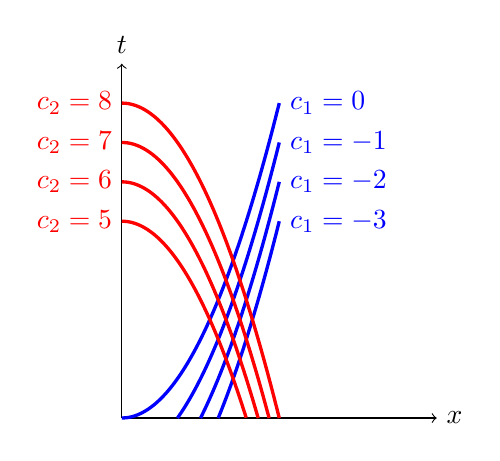
\begin{tikzpicture}
  \draw[->] (0,0) -- (4.,0) node[right] {$x$};
  \draw[->] (0,0) -- (0,4.5) node[above] {$t$};
  \draw[scale=0.5,domain=0:4,smooth,variable=\x,Blue,very thick] plot ({\x},{0.5*\x*\x}) node [right] {$c_1=0 $};
  \draw[scale=0.5,domain=1.4142:4,smooth,variable=\x,Blue,very thick] plot ({\x},{0.5*\x*\x-1}) node [right] {$c_1=-1$};
  \draw[scale=0.5,domain=2:4,smooth,variable=\x,Blue,very thick] plot ({\x},{0.5*\x*\x-2}) node [right] {$c_1=-2$};
  \draw[scale=0.5,domain=2.44948:4,smooth,variable=\x,Blue,very thick] plot ({\x},{0.5*\x*\x-3}) node [right] {$c_1=-3$};
  \draw[scale=0.5,domain=0:3.16,smooth,variable=\x,Red,very thick] plot ({\x},{-0.5*\x*\x+5});
  \node[left,Red] at (0,2.5) {$c_2=5$};
  \draw[scale=0.5,domain=0:3.4641,smooth,variable=\x,Red,very thick] plot ({\x},{-0.5*\x*\x+6});
  \node[left,Red] at (0,3) {$c_2=6$};
  \draw[scale=0.5,domain=0:3.7416,smooth,variable=\x,Red,very thick] plot ({\x},{-0.5*\x*\x+7});
  \node[left,Red] at (0,3.5) {$c_2=7$};
  \draw[scale=0.5,domain=0:4,smooth,variable=\x,Red,very thick] plot ({\x},{-0.5*\x*\x+8});
  \node[left,Red] at (0,4) {$c_2=8$};
\end{tikzpicture}
%%% Local Variables:
%%% mode: latex
%%% TeX-master: "../../mainManuscript"
%%% End:
} \qquad
  \subfloat[Example \ref{ex:charac2}: $\lambda^{1}=1 \: \lambda^2=1/2$]{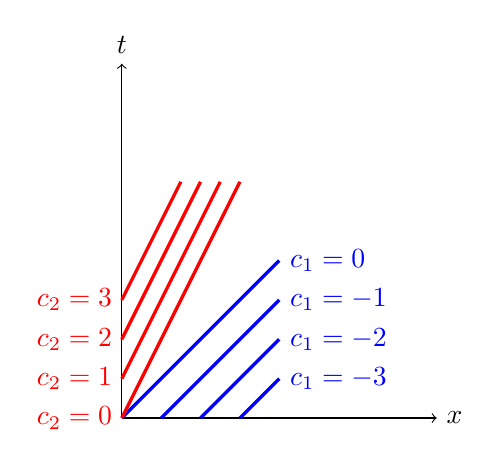
\begin{tikzpicture}
  \draw[->] (0,0) -- (4.,0) node[right] {$x$};
  \draw[->] (0,0) -- (0,4.5) node[above] {$t$};
  \draw[scale=0.5,domain=0:4,smooth,variable=\x,Blue,very thick] plot ({\x},{\x}) node [right] {$c_1=0$};
  \draw[scale=0.5,domain=1.:4,smooth,variable=\x,Blue,very thick] plot ({\x},{\x-1}) node [right] {$c_1=-1$};
  \draw[scale=0.5,domain=2:4,smooth,variable=\x,Blue,very thick] plot ({\x},{\x-2}) node [right] {$c_1=-2$};
  \draw[scale=0.5,domain=3:4,smooth,variable=\x,Blue,very thick] plot ({\x},{\x-3}) node [right] {$c_1=-3$};
  \draw[scale=0.5,domain=0:3,smooth,variable=\x,Red,very thick] plot ({\x},{2*\x});
  \node[left,Red] at (0,0) {$c_2=0$};
  \draw[scale=0.5,domain=-0.:2.5,smooth,variable=\x,Red,very thick] plot ({\x},{2*\x+1});
  \node[left,Red] at (0,0.5) {$c_2=1$};
  \draw[scale=0.5,domain=-0:2,smooth,variable=\x,Red,very thick] plot ({\x},{2*\x+2});
  \node[left,Red] at (0,1) {$c_2=2$};
  \draw[scale=0.5,domain=-0:1.5,smooth,variable=\x,Red,very thick] plot ({\x},{2*\x+3});
  \node[left,Red] at (0,1.5) {$c_2=3$};
\end{tikzpicture}
%%% Local Variables:
%%% mode: latex
%%% TeX-master: "../../mainManuscript"
%%% End:
}
  \caption{Family of base characteristic curves corresponding to the eigenvalues of the first order systems given in examples \ref{ex:charac1} and \ref{ex:charac2}.}
  \label{fig:exampleCharac}
\end{figure}

In analogy with partial differential equations, infinitely many solution to Cauchy problem contain the characteristic curves of a first order partial differential system. As a consequence, one cannot find a unique solution by solving system \eqref{eq:normal_form} if initial conditions are prescribed along a characteristic.  However, an important property of hyperbolic problems that allows to circumvent the difficulties mentioned above will be now highlighted. 
Projecting the quasi-linear system \eqref{eq:1st_order_quasi-linear_syst} onto the \textit{left eigenbasis} or \textit{left characteristic basis}
\begin{equation*}
  \vect{\Lc}^k \( \Absf^t \vect{\Uc}_t + \Absf^x\vect{\Uc}_x \) + \vect{\Lc}^k \vect{\Bc}= \vect{0}
\end{equation*}
and using the definition of left eigenvectors \eqref{eq:eigenvectors} lead to:
\begin{equation*}
  \vect{\Lc}^k  \Absf^t \( \vect{\Uc}_t +\lambda^k \vect{\Uc}_x   \) + \vect{\Lc}^k \vect{\Bc}=\vect{0}
\end{equation*}
In this equation, the \textit{directional derivative} of $\vect{\Uc}$ along the $kth$ characteristic curve arises, namely:
\begin{equation*}
 \ddroit{\Ucb}{t}\lvert_{t\in\phi^k} = \Ucb_t + \lambda^k \Ucb_x   
\end{equation*}
Thus, along a characteristic curve a system of partial differential equations reduces to a system of \textit{Ordinary Differential Equations}:
\begin{equation}
  \label{eq:PDEs_ODEs}
  \vect{\Lc}^k  \Absf^t \(\ddroit{\Ucb}{t} + \Bcb \)=\vect{0}
\end{equation}
This result implies that unlike for non-characteristic, initial conditions can not be prescribed arbitrarily along a characteristic curve but must satisfy equation \eqref{eq:PDEs_ODEs}. 

Use domain of dependence ; theorems \ref{th:integral_surface_generated} and \ref{th:charac_in_integral_surface} to describe the method of characteristic. Then illustrate in with the $3\times 3$ example.

The result that has been obtained in this part is the foundation of the \textit{method of characteristics} that will be developed in what follows. 


\subsubsection*{The method of characteristics}
%%%%%%%%%%%% COMMENTS
% \textit{Domain of dependence, uniqueness.\todo{see \cite[p.424;p.438]{Courant}}}
% notion to investigate \cite[p.408]{Courant}:
% \begin{itemize}
% \item initial data on a characteristic curve can not be prescribed freely but mus satisfy a compatibility condition to be extended into integral strips
% \item discontinuities along characteristic curves only
% \item characteristics are the only possible branch lines of a solution, lines for which the same initial value problem may have several solutions
% \end{itemize}
% If two characteristic curves have a common point, the solution $u(x,t)$ contains those two characteristic curves. 
%%%%%%%%%%%%%%%%%%%%%%%
From now on, the independant variables used so far $x$ and $t$ will explicitly represent  space and time variables respectively, introducing thus the mechanical formalism. Suppose that initial conditions in a one-dimensional domain are given by a function $\Ucb(x,0)=\Ucb_0(x)$. Once we know all the characteristic curves involved in the problem, it is possible to determine the solution at a given point $(x^*,t^*)$ by tracing backward all the characteristic from this point to the $x-$axis.
\begin{figure}[h]
  \centering
  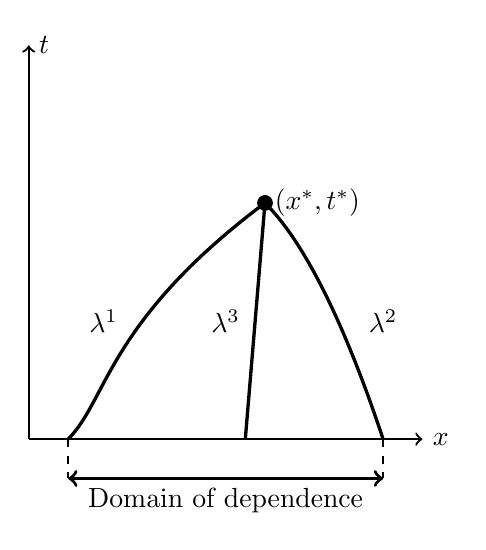
\begin{tikzpicture}
  \draw[thick,->](0,0)--(5,0) node [right] {$x$};
  \draw[thick,->](0,0)--(0,5) node [right] {$t$};
  \fill[black] (3,3) circle (0.1) node [right] {$(x^*,t^*)$};
  \draw[very thick] (0.5,0) .. controls (1.,0.5)and (1,1.5) .. (3.,3);
  \draw[very thick] (4.5,0) .. controls (4.,1.5) and (3.5,2.5) .. (3.,3);
  \draw[very thick] (2.75,0) -- (3.,3);
  \node at (0.95,1.5) {$\lambda^1$};
  \node at (2.5,1.5) {$\lambda^3$};
  \node at (4.5,1.5) {$\lambda^2$};
  \node[below] at (2.50,-0.5) {\text{Domain of dependence}};
  \draw[<->,very thick] (0.5,-0.5) -- (4.5,-0.5) ;
  \draw[dashed,thick] (0.5,0) -- (0.5,-0.5);
  \draw[dashed,thick] (4.5,-0.) -- (4.5,-0.5);
\end{tikzpicture}
%%% Local Variables:
%%% mode: latex
%%% TeX-master: "../../mainManuscript"
%%% End:

  \caption{Example of determination of the solution at a given point for a hyperbolic system of dimension 3 by using the notions of characteristic curves and of domain of dependence.}
  \label{fig:charac_method}
\end{figure}
We know that at least one integral surface contains the three characteristic base curves and the initial curve \todo{uniqueness ?}$\Ucb_0(x)$.
%%% Local Variables:
%%% mode: latex
%%% TeX-master: "../mainManuscript"
%%% End:
